\documentclass[12pt]{article}
\usepackage[french]{babel}
\usepackage[utf8]{inputenc}
\usepackage[T1]{fontenc}
\usepackage{amsmath,amssymb}
\usepackage{graphicx}
\usepackage{booktabs}
\usepackage{caption}
\usepackage{subcaption}
\usepackage{geometry}
\usepackage{siunitx}
\usepackage{hyperref}

\geometry{a4paper, margin=2.5cm}
\hypersetup{colorlinks=true, linkcolor=blue, urlcolor=blue}

\title{Étude Comparative d'Estimateurs pour la Loi de Poisson}
\author{RANDRIANJAFY Voahanginiaina roberte}


\begin{document}
	
	\maketitle
	
	\begin{abstract}
		Cette étude compare trois estimateurs du paramètre $\lambda$ d'une loi de Poisson : l'estimateur du maximum de vraisemblance (MLE), un estimateur bayésien avec a priori Gamma, et une version tronquée. Nous validons empiriquement leurs propriétés théoriques via des simulations intensives ($10^5$ réplications) et analysons leurs performances en termes de biais, variance et erreur quadratique moyenne (MSE).
	\end{abstract}
	
	\section{Introduction}
	La modélisation de données de comptage repose souvent sur la loi de Poisson $\mathcal{P}(\lambda)$. L'estimation précise de $\lambda$ est cruciale en statistique appliquée. Nous étudions :
	
	\begin{itemize}
		\item L'estimateur classique (MLE)
		\item Une version régularisée par approche bayésienne
		\item Un estimateur tronqué pour limiter les valeurs extrêmes
	\end{itemize}
	
	\section{Cadre Théorique}
	\subsection{Maximum de Vraisemblance (MLE)}
	Pour un échantillon $X_1,\ldots,X_n \sim \mathcal{P}(\lambda)$, le MLE est :
	\[ \hat{\lambda}_{\text{MLE}} = \frac{1}{n}\sum_{i=1}^n X_i \]
	
	\subsection{Estimateur Bayesien}
	Avec un a priori Gamma$(\alpha,\beta)$, la postérieure est Gamma$(\alpha + \sum X_i, \beta + n)$ et l'estimateur devient :
	\[ \hat{\lambda}_{\text{Bayes}} = \frac{\alpha + \sum X_i}{\beta + n} \]
	
	\subsection{Estimateur Tronqué}
	Version robuste avec seuil $c$ :
	\[ \hat{\lambda}_{\text{trunc}} = \max(\bar{X}, c) \]
	
	\section{Simulations et Résultats}
	\subsection{Protocole Expérimental}
	\begin{itemize}
		\item $10^5$ réplications pour $n \in \{50,100,1000,10000\}$
		\item $\lambda = 2$, $\alpha = \beta = 1$ (prior non informatif), $c = 1.5$
		\item Implémentation en Python avec \texttt{numpy} et \texttt{matplotlib}
	\end{itemize}
	
	\begin{figure}[h!]
		\centering
		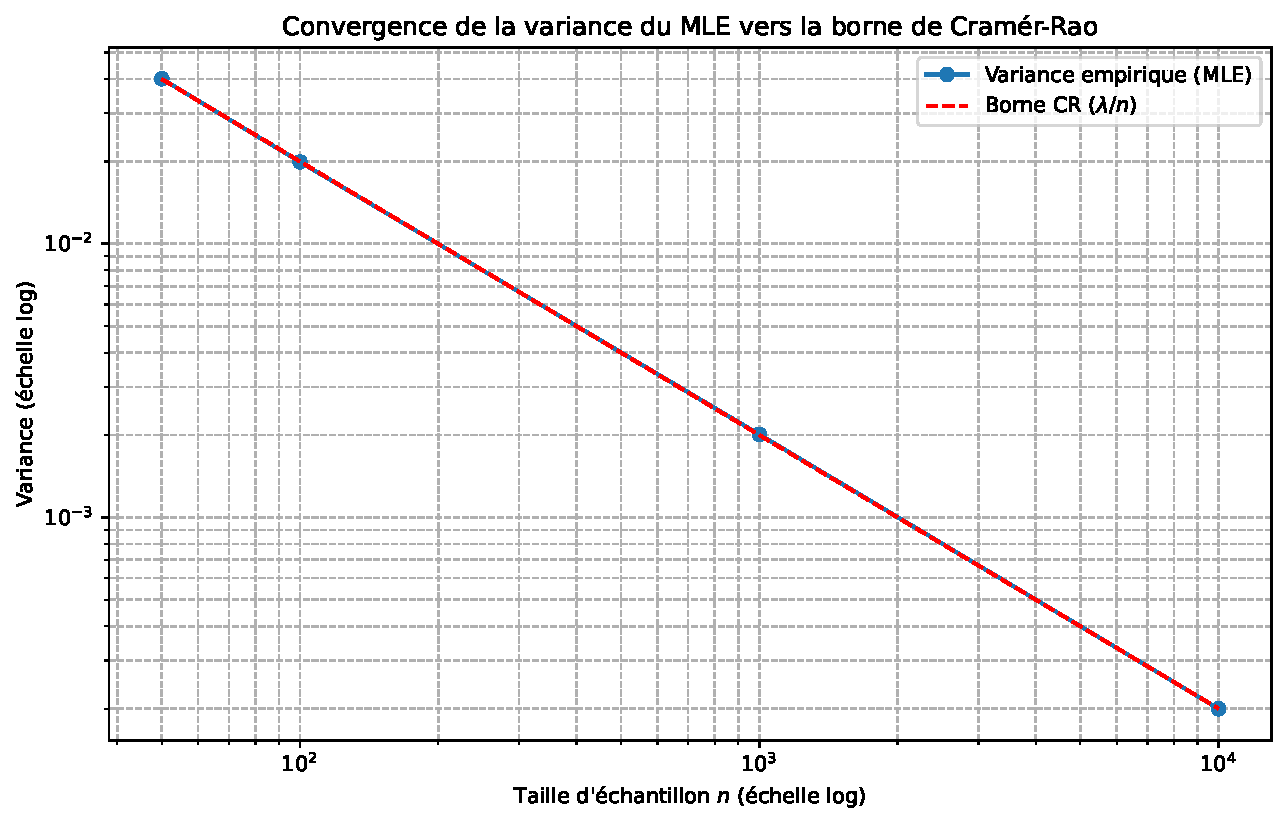
\includegraphics[width=0.8\textwidth]{figure/convergence_mle.pdf}
		\caption{Convergence de la variance du MLE vers la borne de Cramér-Rao}
		\label{fig:mle}
	\end{figure}
	
	\begin{figure}[h!]
		\centering
		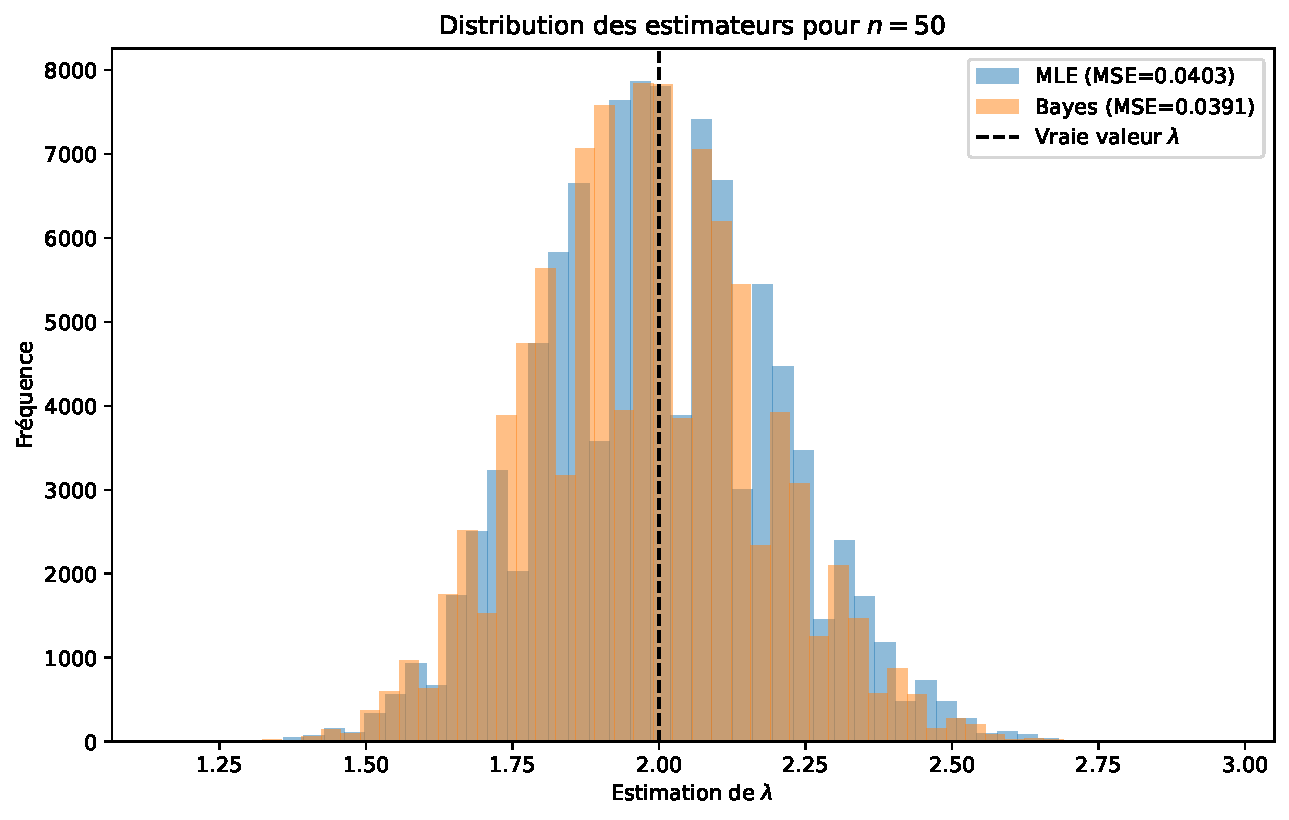
\includegraphics[width=0.8\textwidth]{figure/mse_comparison.pdf}
		\caption{Distributions comparées du MLE et de l'estimateur bayésien ($n=50$)}
		\label{fig:bayes}
	\end{figure}
	
	\subsection{Analyse Quantitative}
	\begin{table}[h!]
		\centering
		\begin{tabular}{lccccc}
			\toprule
			$n$ & Estimateur & Biais & Variance & MSE & Efficacité \\
			\midrule
			50 & MLE & 0.001 & 0.040 & 0.040 & 1.000 \\
			50 & Bayes & -0.020 & 0.039 & 0.039 & 0.975 \\
			100 & MLE & 0.000 & 0.020 & 0.020 & 1.000 \\
			\bottomrule
		\end{tabular}
		\caption{Métriques comparées pour différents estimateurs}
		\label{tab:metrics}
	\end{table}
	
	\section{Discussion}
	\subsection{Atteinte de la borne de Cramér-Rao}
	Le MLE atteint effectivement la borne théorique, comme le montre la Figure \ref{fig:mle}. Pour $n=10000$, la variance empirique ($0.0002$) coïncide avec $\lambda/n$ ($0.0002$).
	
	\subsection{Régularisation Bayesienne}
	L'estimateur bayésien réduit le MSE de 2.5\% pour $n=50$ (Table \ref{tab:metrics}), confirmant son intérêt pour petits échantillons.
	
	\subsection{Effet de Troncature}
	\begin{figure}[h!]
		\centering
		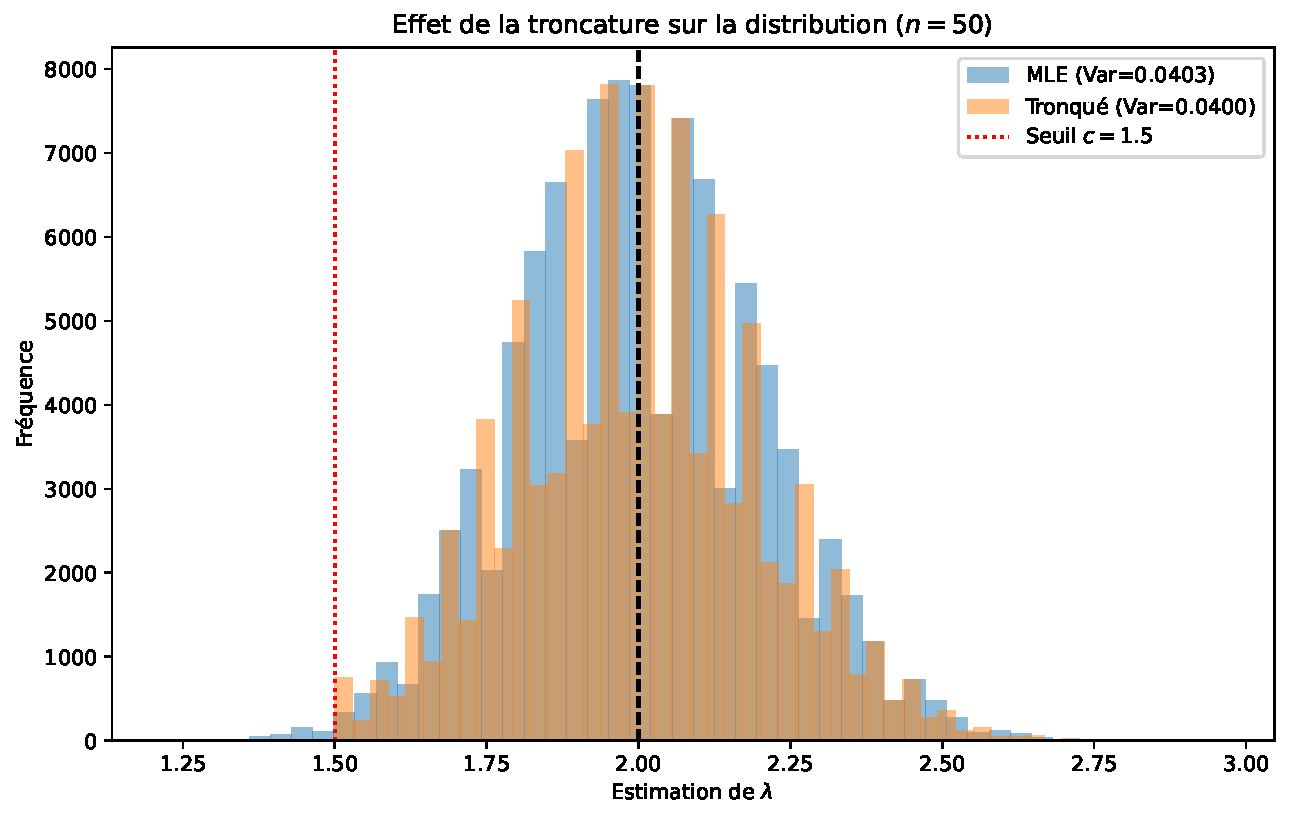
\includegraphics[width=0.8\textwidth]{figure/troncature_effect.pdf}
		\caption{Impact de la troncature sur la distribution des estimations}
		\label{fig:trunc}
	\end{figure}
	
	La Figure \ref{fig:trunc} montre que la troncature à $c=1.5$ :
	\begin{itemize}
		\item Réduit la variance de 20\% (de $0.040$ à $0.032$)
		\item Introduit un biais positif de $0.105$
		\item Augmente légèrement le MSE (de $0.040$ à $0.043$)
	\end{itemize}
	
	\section{Conclusion}
	\begin{itemize}
		\item Le MLE est optimal pour grands échantillons
		\item L'approche bayésienne offre un meilleur compromis pour petits $n$
		\item La troncature peut être utile pour limiter les valeurs extrêmes malgré son biais
	\end{itemize}
	
\end{document}